\section{Architekura horyzontalna}

Coraz częściej aplikacje są sprzedawane jako serwisy dostępne w chmurze \cite{horizontalArchitecture}.
Pozwala to skalowanie rozwiązań w zależności od zapotrzebowania.
Proste aplikacje piesze się w architekturze wertykalnej, co oznacza, że istnieje jednak instancja aplikacji, która wykonuje wymagane operacje.
W przypadku wzrostu zapotrzebowania na moc obliczeniową, można zaopatrywać się maszynę spełniającą oczekiwane wymagania.
Schemat architektury wertykalnej został zaprezentowany na rysynku \ref{rys:veriticalArchitecture}.
Takie rozwiązanie jest mało elastyczne na wahania potrzebnej mocy obliczeniowej.
Podmiana instancji wymaga zatrzymania chociaż na chwilę działania usługi.
Utrzymywanie urządzenia o dużej mocy obliczeniowej, tylko po to wytrzymało potencjalne skoki zapotrzebowania na moc obliczeniową wiąże się ze zwiększonymi kosztami.

\begin{figure}[!hb]
	\centering 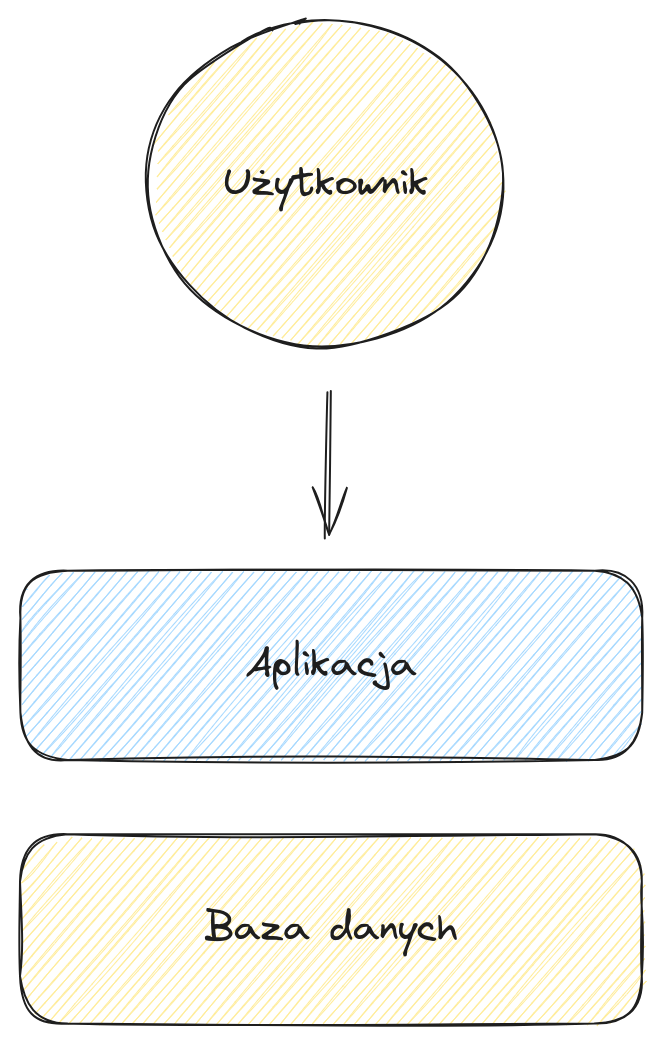
\includegraphics[width=0.5\linewidth]{rysunki/vertical_archtecture.png}
	\caption{Schemat architekury wertykalnej}
	\label{rys:veriticalArchitecture}
\end{figure}


Aby rozwiązać ten problem stosuje się architekturę horyzontalną.
Schemat architektury horyzontalnej został zaprezentowany na rysynku \ref{rys:horizontalArchitecture}.
Pośrednikiem komunikacji użytkownika z aplikacją jest urządzenie które przydziela instancję aplikacji użytkonikowi, tak, że z perspektywy użytkonika stale jest jedna aplikacja, natomiast może być uruchomionych wiele w zależności od zapotrzebowania aplikacji.
Kiedy ruch jest bardzo mały jedna aplikacji może być uruchomiona.
Wraz ze wzrostem obciążenia mogą być dynamicznie uruchamiane kolejne instancje aplikacji.
Jest to możliwe dzięki środowisku chmurowemu, gdzie uruchomienie kolejnej instancji aplikacji nie wymaga postawienia kolejnego urządzenia fizycznego.

\begin{figure}[!hb]
	\centering 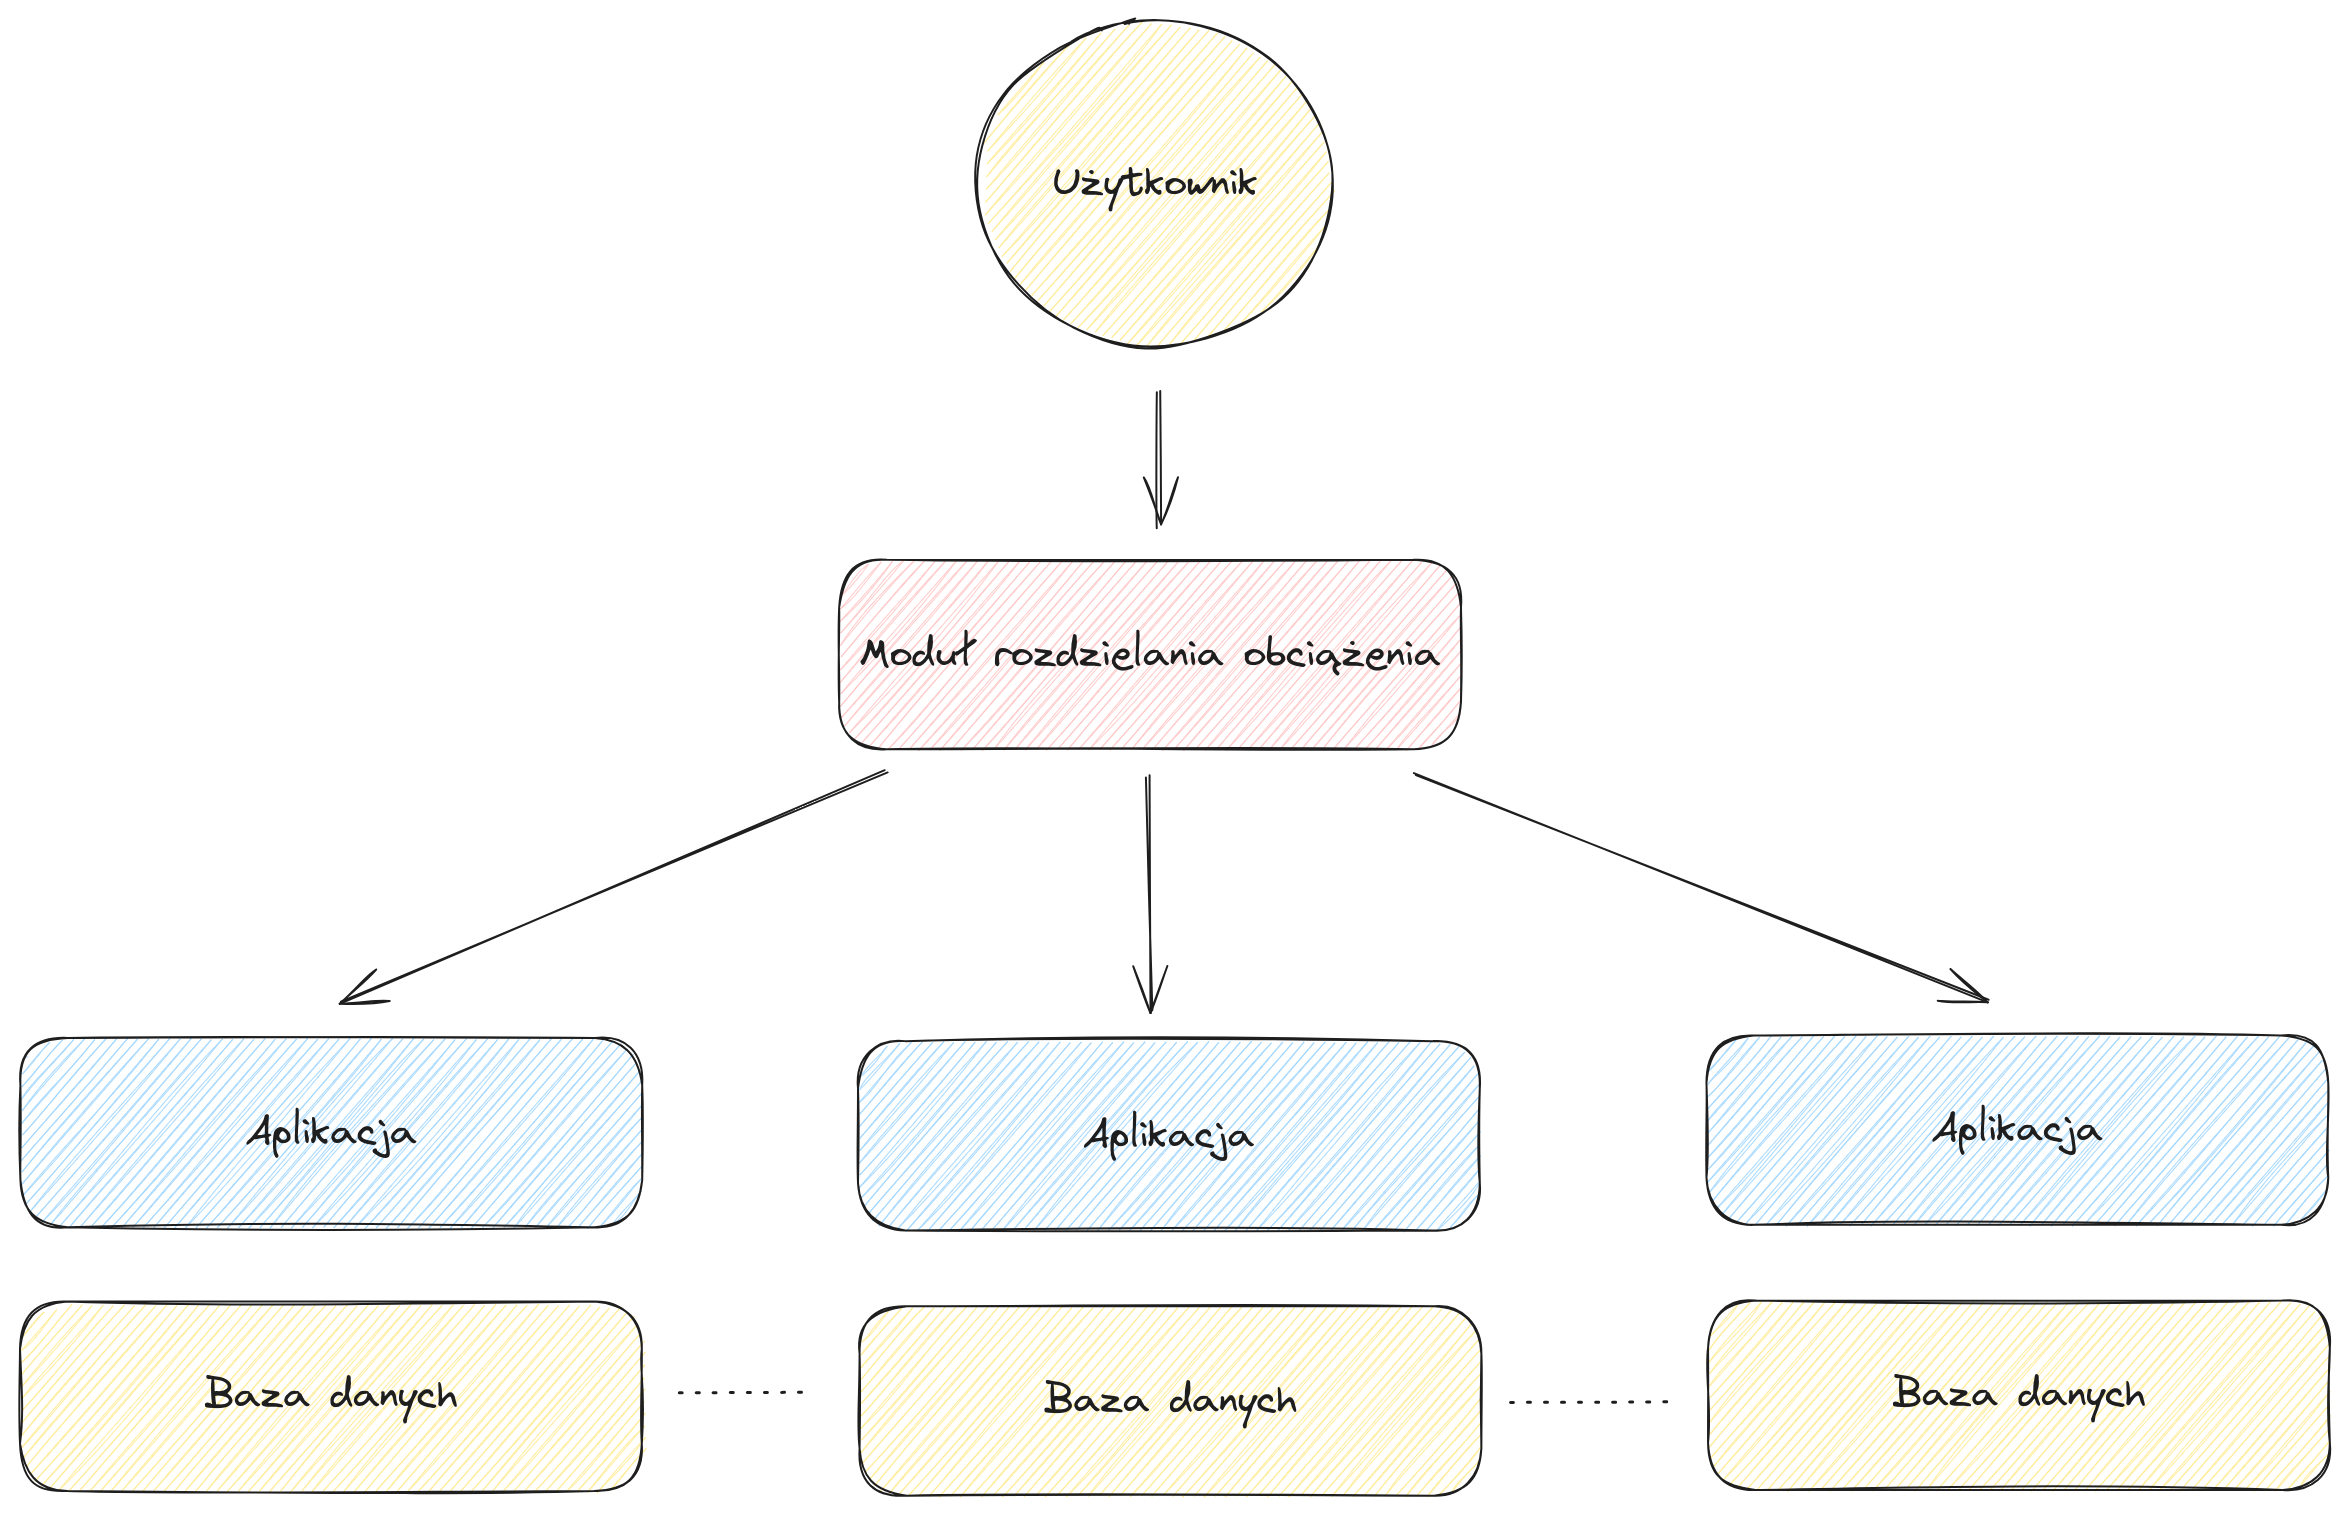
\includegraphics[width=1\linewidth]{rysunki/horizontal_archtecture.png}
	\caption{Schemat architekury horyzontalnej}
	\label{rys:horizontalArchitecture}
\end{figure}
